\documentclass[letterpaper,12pt]{report}

\usepackage[margin=1.0in]{geometry}
\usepackage{multirow}
\usepackage{tikz}
\usepackage{amsmath}
\usepackage{hyperref}
\usepackage{standalone}

\usetikzlibrary{shapes.geometric, arrows, fit}

\setlength\parindent{0pt}

\newcommand{\specialcell}[2][c]{\begin{tabular}[#1]{@{}c@{}}#2\end{tabular}}
\newcommand{\xxx}[1]{{\color{red}\bf #1}}
\newcommand{\AxisRotator}[1][rotate=0]{\tikz [x=0.25cm,y=0.60cm,line
        width=.2ex,-stealth,#1] \draw (0,0) arc (-150:150:1 and 1);}
\newcommand{\github}{\href{https://github.com/utdrobotchess}
        {\textbf{github organization}}}

\begin{document}

\title{\textbf{Chessbot Software Manual}}
\author{Omar Hasan}

\date{\today}
\maketitle

\pagebreak

\section*{Preface}
\label{sec:preface}
The purpose of this document is to both instruct the user on how to operate the
Chessbot as well as inform them about its various quirks. At the time of this
document's writing, the repository that contains the source code for the
Chessbot's processor as well as for the Java app that is used to control it can
be found on our \github. Should the link to the repo change, one might be able
to find it by searching github for an organization named ``utdrobotchess''.\\

If you find anything wrong with this document and you know LaTeX, feel free to
correct it. And finally, if you have any questions or concerns, feel free to
contact our mentor Dr. Nicholas Gans (ngans@utdallas.edu).\\

You can also try to contact one of the team members:\\
\begin{center}
\begin{tabular}{l l}
    Omar Hasan & omarhasan777@gmail.com \\
    Abhi Chennapareddy & ch.abhinav.reddy@gmail.com
\end{tabular}
\end{center}
\addcontentsline{toc}{section}{Preface}

\begin{figure}[!h]
\centering
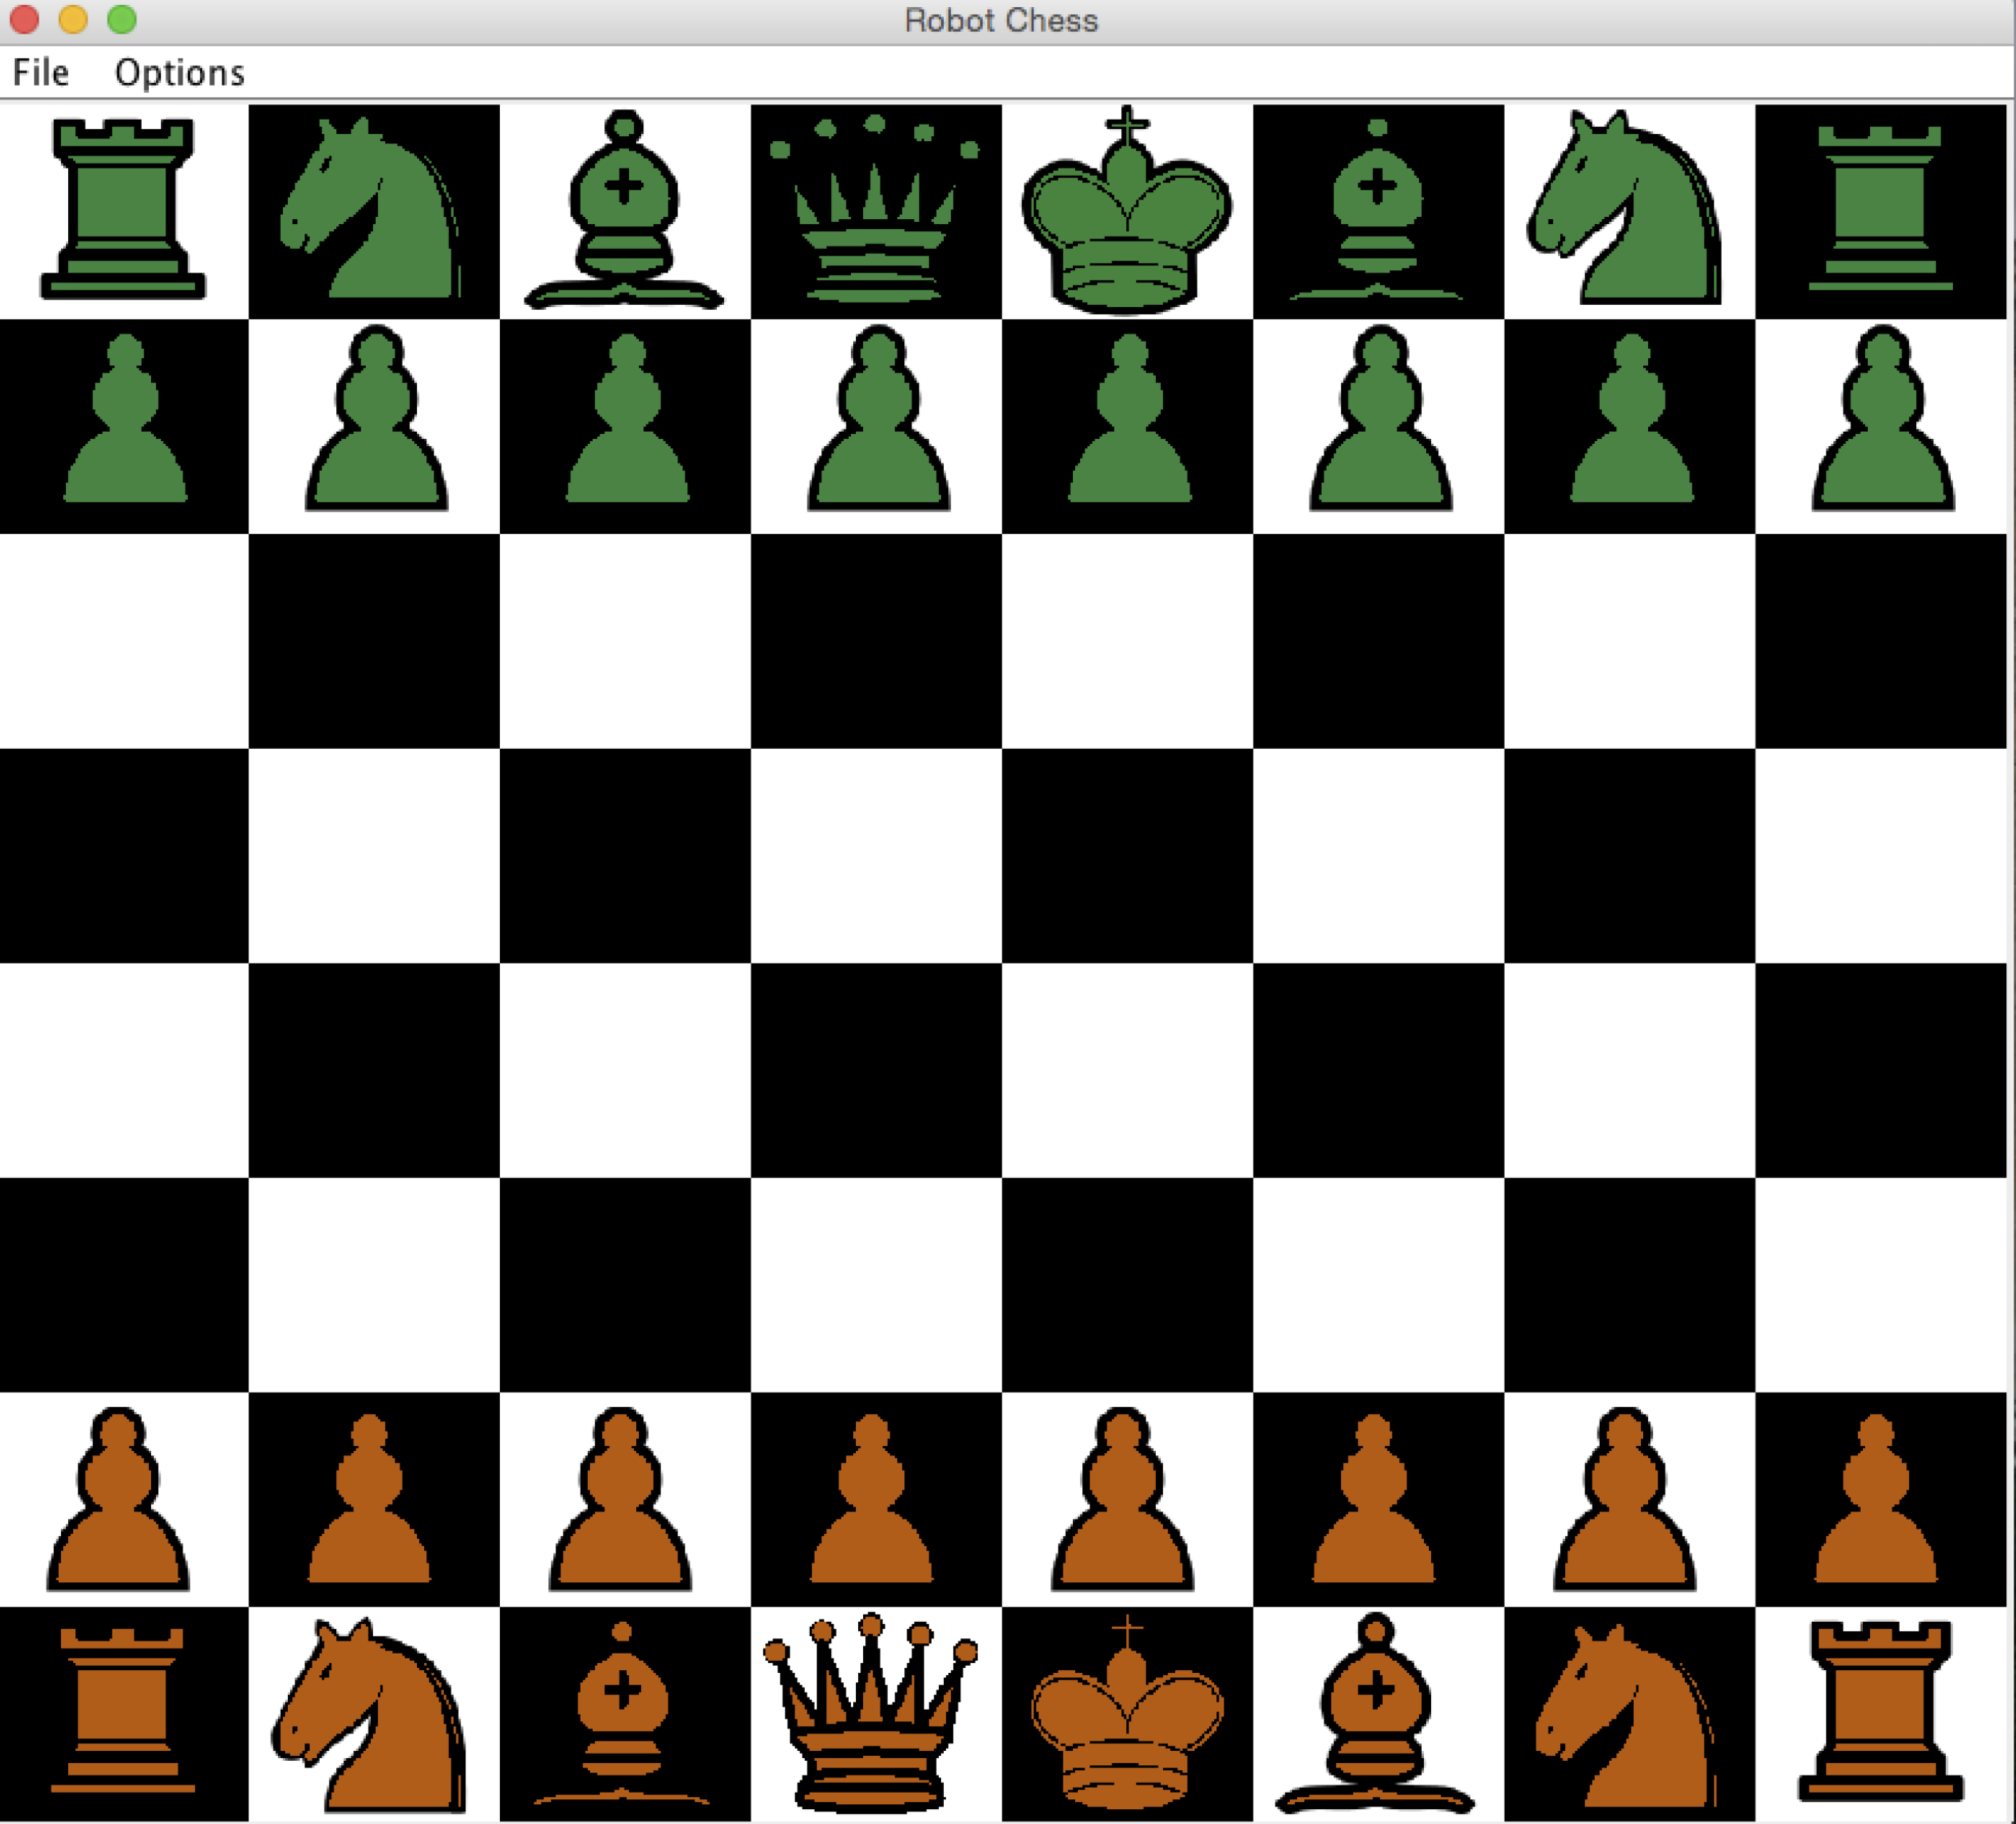
\includegraphics[width=14cm]{./pics/chessboard.jpg}
\end{figure}

\pagebreak
\tableofcontents
\pagebreak

\chapter{Software Overview}
\label{cha:system-design-overview}

\chapter{Future Work}
\label{cha:future-work}

\chapter{Troubleshooting}
\label{cha:troubleshooting}

\end{document}
